\newpage
{\color{gray}\hrule}
\begin{center}
\section{The Numerical Solution}
\bigskip
\end{center}
{\color{gray}\hrule}
\begin{multicols}{2}

\subsection{Trapezoidal Rule}
For a differential equation $$\frac{dy}{dx} = f(x,y)$$ whose solution is $y(x)$, the update equation for trapezoidal method is given by:
\begin{align}
    y_{n+1} = y_n + \frac{h}{2}\left[ f(x_n,y_n) + f(x_{n+1},y_{n+1}) \right]
\end{align}
\subsection{Derivation of Update Equation}
To solve the differential equation numerically using the trapezoidal method, we discretize it as:
\begin{equation}
L \frac{I_{n+1} - I_n}{\Delta t} + R \frac{I_{n+1} + I_n}{2} = \frac{V_{n+1} + V_n}{2}
\end{equation}
Rearranging to isolate $I_{n+1}$:
\begin{equation}
L \frac{I_{n+1} - I_n}{\Delta t} = \frac{V_{n+1} + V_n}{2} - R \frac{I_{n+1} + I_n}{2}
\end{equation}
\begin{equation}
I_{n+1} \left( \frac{L}{\Delta t} + \frac{R}{2} \right) = I_n \left( \frac{L}{\Delta t} - \frac{R}{2} \right) + \frac{V_{n+1} + V_n}{2}
\end{equation}
Defining:
\begin{align}
A &= \frac{2L - R \Delta t}{2L + R \Delta t} \\
B &= \frac{\Delta t}{2L + R \Delta t}
\end{align}
The iterative formula becomes:
\begin{equation}
I_{n+1} = A I_n + B (V_{n+1} + V_n)
\end{equation}
\subsection{Why Trapezoidal?}
\begin{enumerate}
    \item Trapezoidal Rule is a popular method that is most used to solve real-world problems.
    \item It is an A-stable numerical method.
    \item Other popular numerical techniques such as Forward Euler and Backward Euler are first-order accurate, whereas Trapezoidal Rule is second-order accurate.
\end{enumerate}

\subsection{The Code}
\begin{lstlisting}[caption={Code for Numerical Analysis}]
import numpy as np
import matplotlib.pyplot as plt

def square_wave(t, T, alpha):
    return np.array([10 if (time % T) < (alpha * T) else 0 for time in t])

def rl_circuit_response(R, L, T, alpha, t_end, dt=0.00005):
    t = np.arange(0, t_end, dt)
    V = square_wave(t, T, alpha)
    I = np.zeros(len(t))
    A = (2 * L - R * dt) / (2 * L + R * dt)
    B = dt / (2 * L + R * dt)
    for i in range(1, len(t)):
        I[i] = A * I[i - 1] + B * (V[i] + V[i - 1])
    plt.figure(figsize=(10, 5))
    plt.plot(t, I, label="Current (I)")
    plt.xlabel("Time (s)")
    plt.ylabel("Current (A)")
    plt.grid(True)
    plt.legend()
    plt.show()

R = 1
L = 1
T = 1
alpha = 0.5
t_end = 5
dt = 0.00005

rl_circuit_response(R, L, T, alpha, t_end, dt)

\end{lstlisting}

The output generated by the above code is:
\begin{figure}[H]
  \centering
  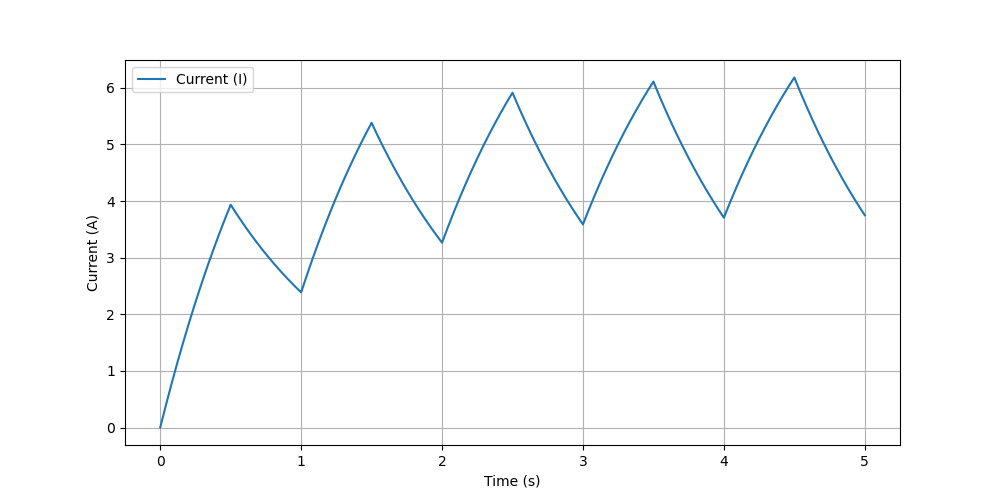
\includegraphics[width=\columnwidth]{sections/4_og.png}
  \caption{Current Response for $R=1\Omega$, $L=1H$, $T=1s$, and $\alpha=0.5$}
\end{figure}

\end{multicols}
